\newcommand{\substxy}[3]{\textcolor{#1}{[x\mapsto {#2}; y\mapsto {#3}]}}
\newcommand{\upperB}{\boxed{o}}
\newcommand{\lowerB}{\boxed{u}}
\newcommand{\landp}{\land_p}
\newcommand{\lorp}{\lor_p}
\newcommand{\implp}{{\implies_{\!\!\!\!p}}}
\newcommand{\timesp}{\times_p}
\newcommand{\topp}{\top_p}
\newcommand{\botp}{\bot_p}
\newcommand{\negp}{\neg_p}
\newcommand{\forallp}{\forall_p}
\newcommand{\existsp}{\exists_p}

\begin{frame}[fragile]
    \frametitle{Agenda}

    \begin{itemize}
        \item Review of choice algebra.
        \item Typing syntax and denotation.
        \item Some interesting examples.
        \item Typing rules.
        \item Future plans.
    \end{itemize}
\end{frame} 

\begin{frame}[fragile]
    \frametitle{Preliminaries}

\begin{definition}[Substitution] 
    A substitution $\sigma: \Code{Var} \rightharpoonup \Code{Value}$ is a partial function (mapping) from variables to resources.
\end{definition}

\begin{definition}[Pointwise Union] $m_1 \times m_2 \doteq \{ \sigma_1 \cup \sigma_2 ~|~ \sigma_1 \in m_1 \land \sigma_2 \in m_2 \}$.
\end{definition}

\begin{definition}[Projection]
    \begin{align*}
    &\Code{Proj}(X, \sigma) \doteq
        \begin{cases}
            \bigcup_{x \in X} [x\mapsto \sigma(x)] & \text{when } X \subseteq \Dom{\sigma} \\
            \text{undefined} & \text{otherwise}
        \end{cases}
    \\&\Code{Proj}(X, m) \doteq
    \begin{cases}
        \bigcup_{\sigma \in m} \{ \Code{Proj}(X, \sigma) \} & \text{when } X \subseteq \Dom{m} \\
        \text{undefined} & \text{otherwise}
    \end{cases}
    \end{align*}
\end{definition}
    
\end{frame}

\begin{frame}[fragile]
    \frametitle{Choice Algebra}

\begin{definition}[Choice Algebra] A choice algebra is a tuple $(M, \mathbf{0}, \mathbf{1}, +, \times)$ where:
    \begin{itemize}
        \item A resource $m$ is a set of substitutions: $\mathcal{P}(\Code{Var} \rightharpoonup \Code{Value})$.
        \item $M$ is the set of resources.
        \item $\mathbf{0}$ is $\emptyset$; $\mathbf{1}$ is $\{\emptyset\}$.
        \item $+$ is the union operation; $\wfvdash m_1 + m_2$ iff $\Dom{m_1} = \Dom{m_2}$.
        \item $\times$ is the pointwise union operation:
        \begin{align*}
        m_1 \times m_2 \doteq \{ \sigma_1 \cup \sigma_2 ~|~ \sigma_1 \in m_1 \land \sigma_2 \in m_2 \}
        \end{align*}
        \item $\leq$ is the partial order on resources:
        \begin{align*}
        m_1 \leq m_2 \doteq
        \begin{cases}
            \exists m_3.\ m_1 \times m_3 = m_2 & \text{when } \Dom{m_1} \subseteq \Dom{m_2} \\
            \text{undefined} & \text{otherwise}
        \end{cases}
        \end{align*}
    \end{itemize}
\end{definition}
    
\end{frame}

\begin{frame}[fragile]
    \frametitle{Pure Propositions}

Assume we have an expressive enough pure propositional logic $\phi: (\Code{Var} \rightharpoonup \Code{Value}) \sarr \Bool$:
\begin{align*}
\phi \doteq \Code{Atom} ~|~ \Dom{X} ~|~ \phi \cap \phi ~|~ \phi \cup \phi ~|~ \phi \setminus \phi ~|~ \phi \times \phi
\end{align*}
where
\begin{itemize}
    \item $\Code{Atom}$ is an atomic proposition, e.g., $\denot{x < 2} = \{[x\mapsto 0], [x\mapsto 1]\}$.
    \item $\Dom{X}$ ensures that all substitutions have the same domain as $X$.
    \item $\phi \cap \psi$ is the intersection of $\phi$ and $\psi$.
    \item $\phi \cup \psi$ is the union of $\phi$ and $\psi$.
    \item $\phi \setminus \psi$ is the difference of $\phi$ and $\psi$.
    \item $\phi \times \psi$ is the pointwise union of $\phi$ and $\psi$.
\end{itemize}

\textbf{Note:} The denotation of $\phi$ ($\denot{\phi}$) is a set of substitutions that satisfy $\phi$; the denotation of ``choice algebra terms'' is a set of resources.

\end{frame}

\begin{frame}[fragile]
    \frametitle{Basic Choice Logic}

\begin{definition}[Basic Choice Logic] Basic choice logic has no approximation; everything needs to be precise.
\end{definition}
\begin{itemize}
    \item $m \models p * q$ iff $\exists m_1, m_2.\ m_1 \times m_2 \leq m \text{ and } m_1 \models p \text{ and } m_2 \models q$.
    \item $m \models p \wand q$ iff $\forall m'. m' \models p  \implies m' \times m \models q$.
    \item $m \models p \oplus q$ iff $\exists m_1, m_2.\ m_1 + m_2 \leq m \text{ and } m_1 \models p \text{ and } m_2 \models q$.
    \item $m \models \phi$ iff $\{\sigma ~|~ \Dom{\sigma} = \Code{FV}(p) \land \sigma(p)\}\leq m$.
    \item $m \models \true$ always; $m \models \false$ \textcolor{red}{iff $m = \mathbf{0}$}.
    \item $m \models p \land q$ iff $m \models p$ and $m \models q$.
    \item $m \models p \implies q$ iff $m \models p$ implies $m \models q$.
    \item $m \models p \lor q$ iff $m \models p$ or $m \models q$.
    \item $m \models \forall x. p$ iff for all $v$, $m \models p[x\mapsto v]$.
    \item $m \models \exists x. p$ iff there exists $v$ such that $m \models p[x\mapsto v]$.
\end{itemize}

\end{frame}


\begin{frame}[fragile]
    \frametitle{Choice Logic with Approximation}

\begin{definition}[Choice Logic with Approximation] We consider two new modalities, $\upperB$ and $\lowerB$.
    \begin{itemize}
        \item $m \models\upperB\phi$ iff $\exists m_1, m'.\ m + m_1 = m' \text{ and } m' \models\phi$.
        \item $m \models\lowerB\phi$ iff $\exists m_1, m'.\ m' + m_1 = m  \text{ and } m' \models\phi$.
    \end{itemize}
\end{definition}

\textbf{Intuition:} They work like the upper and lower bounds of a resource.

\begin{example}
    \begin{itemize}
        \item $\{[x\mapsto 0]\} \models\upperB(x < 2)$.
        \item $\{[x\mapsto 0], [x\mapsto 1], [x\mapsto 2]\} \models\lowerB(x < 2)$.
        \item $\{[x\mapsto 0], [x\mapsto 1], [x\mapsto 2]\} \models\upperB(x < 4) \land \lowerB(x < 2)$.
    \end{itemize}
\end{example}

\end{frame}

\begin{frame}[fragile]
    \frametitle{Normal Form}

\begin{definition}[Approximation Normal Form (AppNF)] The syntax is:
\begin{align*}
    \textbf{Variables} \quad x, y, z  \\
    \textbf{Variable Sets} \quad X, Y, Z \\
    \textbf{Constants} \quad c ::= & () ~|~ \mathbb{B} ~|~ \mathbb{Z} ~|~ ...  \\
    \textbf{Pure Propositions} \quad \phi ::= & \Code{Atom} ~|~ \Dom{X}\\
    & ~|~ \phi \cap \phi ~|~ \phi \cup \phi ~|~ \phi \setminus \phi ~|~ \phi \times \phi \\
    \textbf{Resource Propositions} \quad p,q ::= & \upperB \phi ~|~ \lowerB \phi ~|~ p \land q ~|~ p \lor q ~|~ p \implies q \\
    &~|~ \forall x. p ~|~ \exists x. p ~|~ \true ~|~ \false \\
    &~|~ p * q ~|~ p \oplus q ~|~ p \wand q
\end{align*}
\end{definition}

\end{frame}

\begin{frame}[fragile]
    \frametitle{Properties of Approximation}

\begin{theorem}[Equivalence] Every AppNF formula is equivalent to the original formula.
\end{theorem}

Some clarifications:
\begin{lemma}[Intersection and Union] Consider pure propositions $\phi_1$ and $\phi_2$.
\begin{itemize}
    \item $\upperB \phi_1 \land \upperB \phi_2 \dashv\vdash \upperB(\phi_1 \cap \phi_2)$.
    \item $\upperB \phi_1 \oplus \upperB \phi_2 \dashv\vdash \upperB(\phi_1 \cup \phi_2)$.
    \item $\lowerB \phi_1 \land \lowerB \phi_2 \dashv\vdash \lowerB(\phi_1 \cap \phi_2)$.
    \item $\lowerB \phi_1 \oplus \lowerB \phi_2 \dashv\vdash \lowerB(\phi_1 \cup \phi_2)$.
\end{itemize}
\end{lemma}

\end{frame}

\begin{frame}[fragile]
    \frametitle{Dependent Types and Dependent Pairs}

\textbf{Problem:} The refinement type includes dependent types and dependent pairs. However, we assume $*$ is disjointed.

\begin{align*}
    \lowerB (0 \leq x \leq 3) * \lowerB (0 \leq y \leq x) 
\end{align*}\noindent

\textbf{Question:} What is meaning of the above formula?

\textbf{Idea:} $x$ can cover the range $[0,3]$; whatever what $x$ is chooson, $y$ can be chosen independently to be in the range of $[0,x]$.

\end{frame}

\begin{frame}[fragile]
    \frametitle{Dependent Types and Dependent Pairs}

\begin{figure}
    \centering
    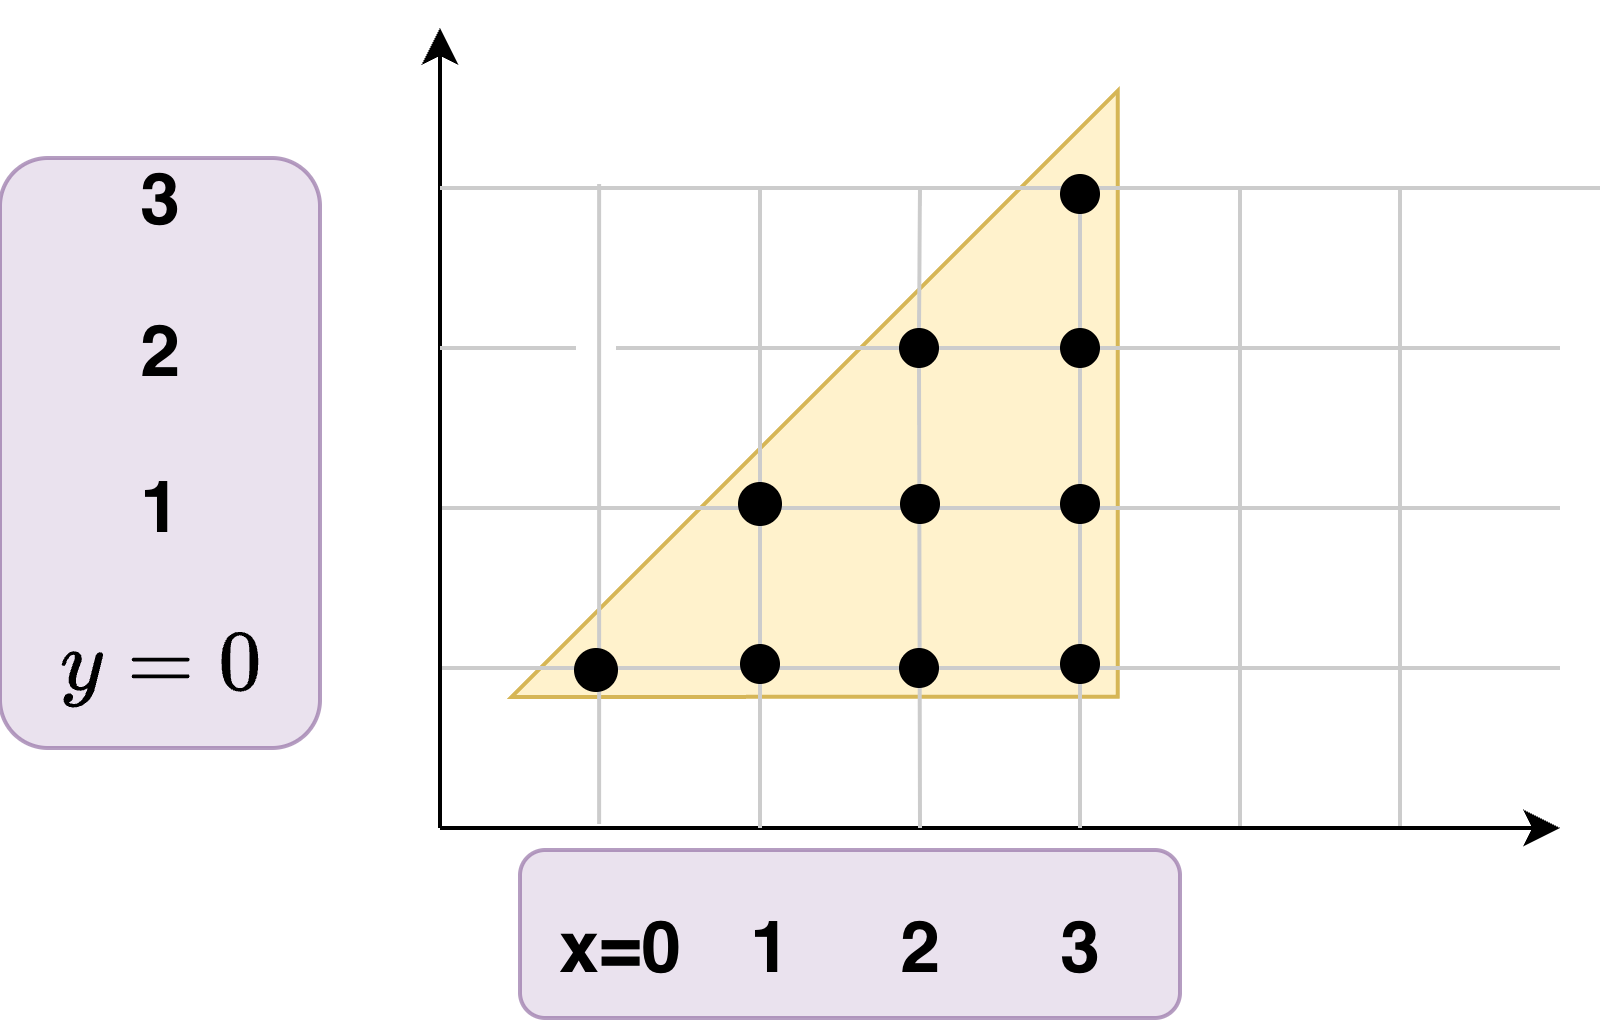
\includegraphics[width=0.8\textwidth]{figures/Ex8.drawio.png}
\end{figure}

\textbf{Example:} $x :: xs$ covers all sorted list when $x$ cover all integers and $xs$ cover all sorted lists \textbf{whose head element is less than $x$}.
\end{frame}


\begin{frame}[fragile]
    \frametitle{Dependent Types and Dependent Pairs}

\textbf{Question:} How to express such a trangle?

\textbf{Problem:} $\times$ can only express rectangle and $\land$ has no limitation on the shape.

\textbf{Idea:} A generalized product operator in monadic way:

\begin{definition}[Monadic Resource]
    The type of substitution is $M \doteq \Code{Var} \rightharpoonup \Code{Value}$.
    The generalized resource $m$ is now has type $M \sarr \mathcal{P}(M)$, where $m$ is a set of substitutions \emph{under given input substitution}.

    Consider a resource application $\sigma = m(\sigma_0)$, we need to make sure that $m$ cannot change the $\sigma_0$ (read only), thus we add constraint:
    \begin{align*}
        \forall \sigma_0, \Dom{\sigma_0} \land \Dom{m(\sigma_0)} 
    \end{align*}
    which means that $m$ cannot produce substitutions with different domain.

    We still defined $\Dom{m}$ as its output domain.
\end{definition}


\end{frame}

\begin{frame}[fragile]
    \frametitle{Dependent Types and Dependent Pairs}

\begin{definition}[Monadic Resource Algebra]

    The generalized operators are defined as:
    \begin{align*}
        m_1 + m_2 &\doteq \lambda \sigma_0. m_1(\sigma_0) \cup m_2(\sigma_0) 
        \\m_1 \times m_2 &\doteq \lambda \sigma_0. \{ \sigma_1 \cup \sigma_2 ~|~ \sigma_1 \in m_1(\sigma_0) \land \sigma_2 \in m_2(\sigma_0 \cup \sigma_1)  \}
    \end{align*}
\end{definition}

\begin{example}
$m_1 = \{ (\emptyset, [x\mapsto 0]), (\emptyset, [x\mapsto 1]), (\emptyset, [x\mapsto 2]) \}$
$m_2 = \{ ([x\mapsto 0], [y\mapsto 0]), ([x\mapsto 1], [y\mapsto 0]), ([x\mapsto 1], [y\mapsto 1]), ... \}$
$m_1 \times m_2 = \{ (\emptyset, [x\mapsto 0;y\mapsto 0]), (\emptyset, [x\mapsto 1;y\mapsto 0]), (\emptyset, [x\mapsto 1;y\mapsto 1]), ... \}$
\end{example}

\end{frame}

\begin{frame}[fragile]
    \frametitle{Dependent Types and Dependent Pairs}

\textbf{Problem:} We lose the commutativity of $\times$.

\textbf{Idea:} We keep the resource and logic simple, the bindings in type context are not resources, but monadic resources.

\begin{example}
    \begin{itemize}
    \item $\denot{x{:}\urt{\Int}{0 \leq x \leq 3}} = \{ (\emptyset, [x\mapsto 0]), (\emptyset, [x\mapsto 1]), (\emptyset, [x\mapsto 2]) \}$
    \item $\denot{y{:}\urt{\Int}{0 \leq y \leq x}} = \{ ([x\mapsto 0], [y\mapsto 0]), ([x\mapsto 1], [y\mapsto 0]), ([x\mapsto 1], [y\mapsto 1]), ... \}$
    \item $\denot{x{:}\urt{\Int}{0 \leq x \leq 3} * y{:}\urt{\Int}{0 \leq y \leq x}} = \{ (\emptyset, [x\mapsto 0;y\mapsto 0]), (\emptyset, [x\mapsto 1;y\mapsto 0]), (\emptyset, [x\mapsto 1;y\mapsto 1]), ... \}$
    \end{itemize}
    \end{example}

\end{frame}

\begin{frame}[fragile]
    \frametitle{Modal Types}

\begin{definition}[Modal Type] The types have the following syntax:
\begin{align*}
    \textbf{Pure Qualifiers} \quad \phi ::= &\; \Code{lit} ~|~ \top ~|~ \bot ~|~ \neg \phi ~|~ \phi \land \phi ~|~ \phi \lor \phi\\
    & ~|~ \phi \impl \phi ~|~ \phi \times \phi ~|~ \forall x. \phi ~|~ \exists x. \phi \\
    \textbf{Refinement Types} \quad \tau ::= &\; \ort{b}{\phi} ~|~ \urt{b}{\phi} ~|~ \tau \oplus \tau \\
    % &~|~ (x{:}\tau, \tau) ~|~ (x{:}\tau * \tau) \\
    &~|~ x{:}\tau \sarr \tau ~|~ x{:}\tau \wand \tau ~|~ x{:}b \garr \tau
    \\\textbf{Type Context} \quad \Gamma ::= &\; \emptyset ~|~ x{:}\tau ~|~ \Gamma \sep \Gamma ~|~ \Gamma, \Gamma
\end{align*}
\end{definition}

\begin{itemize}
    \item $\phi$ is similar to the pure propositions in AppNF. Thus $\land$ and $\lor$ are the intersection ($\cap$) and union ($\cup$) of pure propositions.
    \item The empty type context $\emptyset$ is the unit resource $\textbf{1}$.
\end{itemize}

\end{frame}

\begin{frame}[fragile]
    \frametitle{Type Denotation}

We interpret terms and qualifiers as atomic propositions in choice logic.

\begin{definition}[Qualifier Interpretation] The qualifier interpretation $\denot{\phi}$ is the set of substitutions that satisfy $\phi$: $\denot{\phi} \doteq \{\sigma ~|~ \sigma(\phi) \}$.
\end{definition}

\begin{definition}[Term Interpretation] The term interpretation $\denot{\vnu = e}$ is a set of singleton substitutions where $\vnu$ is mapped to all values $e$ can reduce to: $\denot{\vnu = e} \doteq \{[\vnu \mapsto v] ~|~ \mstep{e}{v} \}$.
\end{definition}

\end{frame}

\begin{frame}[fragile]
    \frametitle{Type Annotation Interpretation}

We interpret type annotations as formulae in choice logic.

\begin{definition}[Type Annotation Interpretation] We interpret $x:\tau$ as:
\begin{itemize}
    \item $\denot{e : \ort{b}{\phi}} \doteq \denot{\vnu = e}\impl \upperB \denot{\phi} $.
    \item $\denot{e : \urt{b}{\phi}} \doteq \denot{\vnu = e}\impl \lowerB \denot{\phi} $.
    \item $\denot{e : x{:}\tau_x \sarr \tau} \doteq \forall e_x. \denot{e_x : \tau_x} \implies \denot{e_x : \tau_x} \land \denot{(e\;e_x) : \bigoplus_{\mstep{e_x}{v_x} } \tau[x\mapsto v_x]} $.
    \item $\denot{e : x{:}\tau_x \wand \tau} \doteq \forall e_x. \denot{e_x : \tau_x} \wand \denot{(e\;e_x) : \bigoplus_{\mstep{e_x}{v_x} } \tau[x\mapsto v_x]} $.
    \item $\denot{e : \tau_1 \oplus \tau_2} \doteq \denot{e : \tau_1} \oplus \denot{e : \tau_2} $.
\end{itemize}
\end{definition}

\textbf{Note 1:} The $\oplus$ in function types allows us to precisely describe inhabitant behaviours. Under- or over-approximation depends on the modalities of the parameter and return types.

\end{frame}

\begin{frame}[fragile]
    \frametitle{Type Annotation Interpretation}

\textbf{Note 2:} The function type has no approximation (otherwise it would absorb the modalities of the parameter and return types).

\begin{example} Let $\tau_x = \Unit$ and $\tau = \urt{\Int}{1 \leq \vnu \leq 2}$. The denotation of $\denot{f : x{:}\tau_x \sarr \tau}$ is
    \begin{align*}
        \{ \{f \mapsto \lambda ().1, f\mapsto\lambda ().2\} \;; \{f \mapsto \lambda ().1, f\mapsto\lambda ().2 , f\mapsto\lambda ().3\} \;; ... \}
    \end{align*}
The $\denot{f : \upperB (x{:}\tau_x \sarr \tau)}$ makes $f$ unconstrained, and $\denot{f : \lowerB (x{:}\tau_x \sarr \tau)}$ is unchanged.
 \end{example}

\end{frame}

\begin{frame}[fragile]
    \frametitle{Type Annotation Interpretation}

\textbf{Note 3:} More compositionally: the parameter type is quantified with $\forall$; the meaning of $\exists$ is expressed by the modality of the parameter type.

\begin{example} Consider $\denot{\lambda x.x : x{:}\urt{\Int}{1 \leq \vnu \leq 2} \sarr \urt{\Int}{\vnu = 1}}$ which will be interpreted as
\begin{align*}
    \forall e_x. \denot{e_x : \urt{\Int}{1 \leq \vnu \leq 2}} \implies \denot{(\lambda x.x\;e_x) : \urt{\Int}{\vnu = 1}}
\end{align*}
The formula above is equivalent to
\begin{align*}
    &\forall e_x. \denot{e_x : \urt{\Int}{1 \leq \vnu \leq 2}} \implies \denot{e_x : \urt{\Int}{\vnu = 1}}
    \\\iff&\forall e_x. (\denot{\vnu = e_x} \impl \lowerB (1 \leq \vnu \leq 2)) \impl (\denot{\vnu = e_x} \impl \lowerB (\vnu = 1))
    \\\iff&\forall e_x. \denot{\vnu = e_x} \impl \lowerB (1 \leq \vnu \leq 2)\impl \lowerB (\vnu = 1)
\end{align*}
 \end{example}

\end{frame}

\begin{frame}[fragile]
    \frametitle{Type Denotation}

\begin{definition}[Type Context Interpretation] We interpret $\Gamma$ as:
\begin{itemize}
    \item $\denot{\emptyset} \doteq \lambda \sigma. \true$.
    \item $\denot{x{:}\tau} \doteq \lambda \sigma.\denot{x : \sigma(\tau)} $.
    \item $\denot{\Gamma_1, \Gamma_2} \doteq \lambda \sigma_0. \denot{\Gamma_1}(\sigma_0) \land \denot{\Gamma_2} (\sigma_0) $.
    \item $\denot{\Gamma_1 \sep \Gamma_2} \doteq \lambda \sigma_0. \denot{\Gamma_1}(\sigma_0) \sep \denot{\Gamma_2} (\sigma_0) $.
\end{itemize}
\end{definition}

\begin{definition}[Type Denotation] $\Code{Denot}_\Gamma(\tau) \doteq \{e ~|~ \denot{\Gamma}(\emptyset) \models \denot{e : \tau} \}$.
\end{definition}

\end{frame}

\begin{frame}[fragile]
    \frametitle{Recall: three possible modalities of function application}
Consider type-checking a function application $f\;x$ under type context $x{:}\urt{\Int}{\top}$, that is,
\begin{align*}
    f{:}?, x{:}\urt{\Int}{\top} \sarr f\;x : ?
\end{align*}\noindent
We assume that the result of $f\;x$ can cover all integers; however, there are still three possible situations.
\begin{itemize}
    \item Situation 1: after application, $x$ loses its coverage.
    \item Situation 2: after application, $x$ retains its coverage but is entangled with the result.
    \item Situation 3: after application, $x$ retains its coverage and is independent of the result.
\end{itemize}

\end{frame}

\begin{frame}[fragile]
    \frametitle{Function Type Examples}

\begin{example}[Situation 1 (Incorrectness Type)] $\vdash f : x{:}\urt{\Int}{\top} \wand \urt{\Int}{\top}$.
\begin{itemize}
    \item Type denotation $\denot{f: x{:}\urt{\Int}{\top} \wand \urt{\Int}{\top}}$:
    \begin{align*}
        \forall e_x. \denot{e_x : \urt{\Int}{\top}} \wand \denot{(f\;e_x) : \urt{\Int}{\top}}
    \end{align*}
    \item Consider $e_x = x$, and we have $\{[x\mapsto n] ~|~ n \in \mathbb{Z} \} \models e_x : \urt{\Int}{\top}$. 
    \item According to the definition of $\wand$, the choice used in $\denot{(f\;e_x) : \urt{\Int}{\top}}$ should be disjoint from the choice used in $\denot{e_x : \urt{\Int}{\top}}$.
    \item If we use $\denot{e_x : \urt{\Int}{\top}} \wand \denot{(f\;x) : \urt{\Int}{\top}}$ during application proof, we cannot prove $\denot{x : \urt{\Int}{\top}}$ anymore.
    \item Thus, in the typing of $(f\;e_x)$, it looks as if $x$ is consumed.
\end{itemize}
\end{example}

\end{frame}

\begin{frame}[fragile]
    \frametitle{More Function Type Examples}

\begin{example}[Situation 1] Concrete example $f \doteq \lambda x. \zif{x == 0}{\Code{int\_gen()}}{\Code{err}}$:
    \begin{align*}
        &f : x{:}\urt{\Int}{\top} \wand \urt{\Int}{\top}
    \\ \iff &\forall e_x. \denot{e_x : \urt{\Int}{\top}} \wand \denot{(f\;e_x) : \urt{\Int}{\top}}
    \\ \iff &\forall e_x. (\denot{\vnu = e_x} \impl \lowerB \Dom{\{x\}}) \wand \denot{(f\;e_x) : \urt{\Int}{\top}}
    \\ \iff &\lowerB \Dom{\{x\}} \wand \denot{(f\;x) : \urt{\Int}{\top}}
    \\ \iff &\lowerB \Dom{\{x\}} \wand \denot{\zif{x == 0}{\Code{int\_gen()}}{\Code{err}} : \urt{\Int}{\top}}
    \\ \iff &\lowerB \Dom{\{x\}} \wand 
    \\ & \quad (\upperB (x = 0) \land \Dom{\{\vnu\}} \oplus  \upperB (x \neq 0) \land \bot) \impl \lowerB \Dom{\{\vnu\}}
    \\ \iff &(x = 0 * \Dom{\{\vnu\}}) \models \lowerB \Dom{\{\vnu\}} \text{ and } 
    \\ &(\lowerB (x \neq 0) * \bot) \models \lowerB \bot  
    \end{align*} 
\end{example}

\end{frame}

% \begin{frame}[fragile]

%     \begin{figure}[h]
%         \centering
%         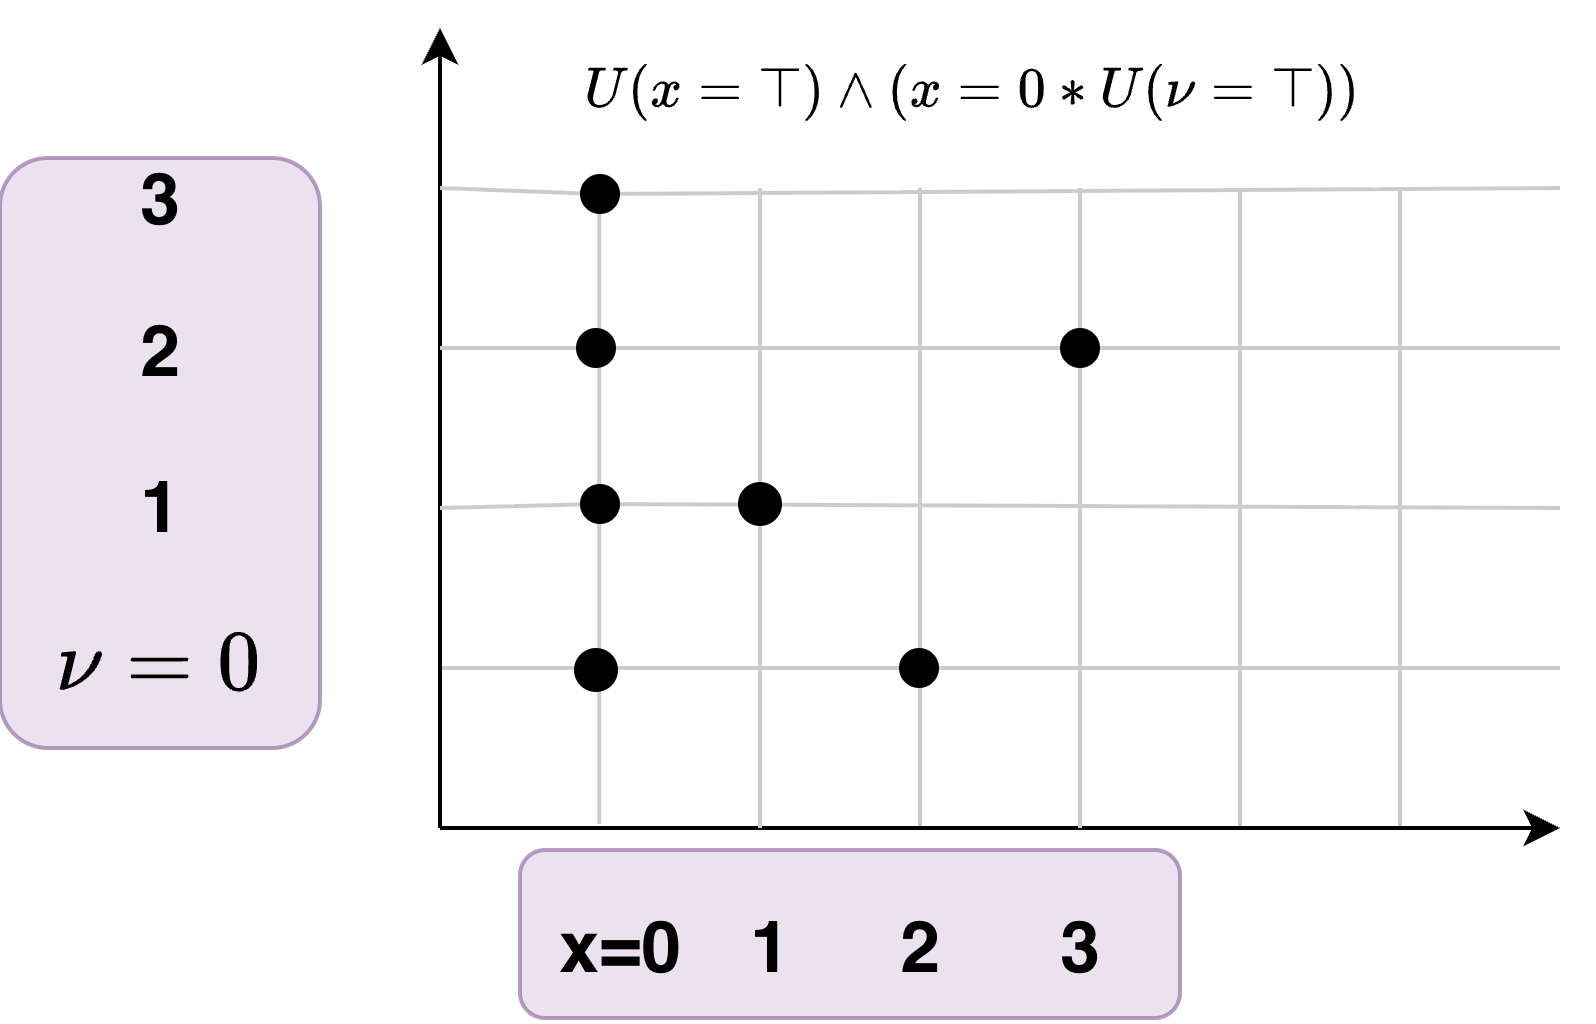
\includegraphics[width=0.8\textwidth]{figures/Ex7.drawio.png}
%         \caption{Situation 1}
%     \end{figure}
% \end{frame}

\begin{frame}[fragile]
    \frametitle{Function Type Examples}

\begin{example}[Situation 2 (Dependent Under-Type)] $\vdash f : x{:}\urt{\Int}{\top} \sarr \urt{\Int}{\top}$.
\begin{itemize}
    \item Type denotation $\denot{f: x{:}\urt{\Int}{\top} \sarr \urt{\Int}{\top}}$:
    \begin{align*}
        \forall e_x. \denot{e_x : \urt{\Int}{\top}} \impl \denot{e_x : \urt{\Int}{\top}} \land \denot{(f\;e_x) : \urt{\Int}{\top}}
    \end{align*}
    \item Consider $e_x = x$, and we have $\{[x\mapsto n] ~|~ n \in \mathbb{Z} \} \models e_x : \urt{\Int}{\top}$. 
    \item According to the definition of $\sarr$, the choice used in $\denot{(f\;e_x) : \urt{\Int}{\top}}$ can be the same as the choice used in $\denot{e_x : \urt{\Int}{\top}}$.
    \item The coverage of $x$ and coverage of the result cannot be used together (not disjointed).
\end{itemize}
\end{example}

\end{frame}

\begin{frame}[fragile]
    \frametitle{More Function Type Examples}

\begin{example}[Situation 2] Concrete example $f \doteq \lambda x. x$:
    \begin{align*}
        &f : x{:}\urt{\Int}{\top} \sarr \urt{\Int}{\top}
    \\ \iff &\forall e_x. \denot{e_x : \urt{\Int}{\top}} \impl \denot{e_x : \urt{\Int}{\top}} \land \denot{(f\;e_x) : \urt{\Int}{\top}}
    \\ \iff &\forall e_x. (\denot{\vnu = e_x} \impl \lowerB \Dom{\{x\}}) \impl \denot{e_x : \urt{\Int}{\top}} \land \denot{(f\;e_x) : \urt{\Int}{\top}}
    \\ \iff &\lowerB \Dom{\{x\}} \impl \lowerB \Dom{\{x\}} \land \denot{(f\;x) : \urt{\Int}{\top}}
    \\ \iff &\lowerB \Dom{\{x\}} \impl \lowerB \Dom{\{x\}} \land \lowerB \Dom{\{x\}}
    \end{align*} 
\end{example}

\end{frame}

\begin{frame}[fragile]
    \frametitle{More Function Type Examples}

\begin{example}[Situation 2] Concrete example $f \doteq \lambda x. \zif{x == 0}{\Code{int\_gen()}}{\Code{err}}$:
    \begin{align*}
        &f : x{:}\urt{\Int}{\top} \sarr \urt{\Int}{\top}
    \\ \iff &\lowerB \Dom{\{x\}} \impl 
    \\ & \quad (\upperB (x = 0) \land \Dom{\{\vnu\}} \oplus  \upperB (x \neq 0) \land \bot) \impl \lowerB \Dom{\{x\}} \land \lowerB \Dom{\{\vnu\}}
    \\ \iff &(x = 0 \land \Dom{\{\vnu\}}) \models x=0 \land \lowerB \Dom{\{\vnu\}} \text{ and } 
    \\ &(\lowerB (x \neq 0) \land \bot) \models ??
    \end{align*} 
\end{example}

\textbf{Why failed?} We cannot find a partition ($+$) of resource to make both cases hold.

\end{frame}

\begin{frame}[fragile]
    \frametitle{Function Type Examples}

\begin{example}[Situation 3 (Coverage Type)] $\vdash f : x{:}\ort{\Int}{\top} \sarr \urt{\Int}{\top}$.
\begin{itemize}
    \item Type denotation $\denot{f: x{:}\ort{\Int}{\top} \sarr \urt{\Int}{\top}}$:
    \begin{align*}
        \forall e_x. \denot{e_x : \ort{\Int}{\top}} \sarr \denot{(f\;e_x) : \urt{\Int}{\top}}
    \end{align*}
    \item Note that for all $n \in \mathbb{Z}$, $n : \ort{\Int}{\top}$ holds. Thus, the formula above is equivalent to
    \begin{align*}
        \forall n{:}\Int. \denot{(f\;n) : \urt{\Int}{\top}}
    \end{align*}
    \item The coverage of $(f\;n)$ does not require additional resources.
    \item Thus we can have both coverage of $x$ and coverage of the result.
\end{itemize}
\end{example}

\end{frame}

\begin{frame}[fragile]
    \frametitle{Higher-order Example}

\begin{minted}[xleftmargin=5pt, numbersep=4pt, linenos = true, fontsize = \footnotesize, escapeinside=??]{OCaml}
let rec find_all (f: int -> bool) (l: int list): int list =
    match l with
    | [] -> []
    | x :: xs -> if f x then x :: (find f xs)  else find f xs
\end{minted}

When return a non-empty list?
\begin{align*}
    \vdash \Code{find} : &f{:}(\urt{\Int}{\top} \wand \urt{\Int}{\vnu}) \sarr \Code{l}{:}\urt{\List[\Int]}{\top} \sarr 
    \\&\ort{\Int}{\neg \I{empty}(\vnu) }
\end{align*}\noindent

When return an empty list?
\begin{align*}
    \vdash \Code{find} : &f{:}(\ort{\Int}{\top} \sarr \ort{\Int}{\vnu}) \sarr \Code{l}{:}\urt{\List[\Int]}{\top} \sarr 
    \\&\ort{\Int}{\I{empty}(\vnu) }
\end{align*}\noindent

Limitation: exists a function type of $f$, cannot be expressed.

Limitation: Precise correctness requires refering $f$ in qualifier logic.

\end{frame}

\begin{frame}[fragile]
    \frametitle{Datatype and dependent pair}

Definition of $\I{sorted}$ list:
\begin{align*}
    \I{sorted}(\vnu) : \Code{l} = [] \lor (\exists x.\exists xs.\Code{l} = x::xs \land x \leq \Code{hd}(xs) \land \I{sorted}(xs))
\end{align*}\noindent

\textbf{Problem:} What is the type of $\Code{cons}$?
\begin{align*}
    \vdash \Code{cons} : (\urt{\Int}{\top} * \urt{\List[\Int]}{\I{sorted}(\vnu)}) \sarr \urt{\List[\Int]}{\I{sorted}(\vnu)}
\end{align*}\noindent
Correct, however, it is too strong.
\begin{align*}
    \vdash \Code{cons} : (\urt{\Int}{\top} , \urt{\List[\Int]}{\I{sorted}(\vnu)}) \wand \urt{\List[\Int]}{\I{sorted}(\vnu)}
\end{align*}\noindent
Incorrect: $\{(\I{hd}(x), l)~|~ \I{sorted}(l) \}$ can only cover lists where the first two elements are equal.
\begin{align*}
    \vdash \Code{cons} : &x{:}\urt{\Int}{\top} \wand \urt{\List[\Int]}{x\leq\I{hd}(\vnu) \land \I{sorted}(\vnu)} 
    \\&\sarr \urt{\List[\Int]}{\I{sorted}(\vnu)}
\end{align*}\noindent

\end{frame}

\begin{frame}[fragile]
    \frametitle{Datatype and dependent pair}

    \textbf{Question:} What happens when we try to pattern match a sorted list?

    \begin{align*}
        &l{:}\urt{\List[\Int]}{\I{sorted}(\vnu)} \vdash \mykw{match}\; l\; \mykw{with} \; ...
        % \\&l{:}\urt{\List[\Int]}{\I{sorted}(\vnu)}, 
        % \\&\quad (x{:}\urt{\Int}{\top} * xs{:}\urt{\List[\Int]}{x\leq\I{hd}(\vnu) \land \I{sorted}(xs)}) &\vdash xs \; ...
        \\&l{:}\urt{\List[\Int]}{\I{sorted}(\vnu)} * 
        \\&\quad (x{:}\urt{\Int}{\vnu = \I{hd}(l)} * xs{:}\urt{\List[\Int]}{\I{tl}(l,\vnu)}) &\vdash xs \; ...
        \\&l{:}\urt{\List[\Int]}{\I{sorted}(\vnu)} * 
        \\&\quad xs{:}\urt{\List[\Int]}{\I{tl}(l,\vnu)} &\vdash xs \; ...
        \\&xs{:}\urt{\List[\Int]}{\exists l. \I{sorted}(l) \land \I{tl}(l,\vnu) = xs} &\vdash xs \; ...
    \end{align*}\noindent

    \textbf{Idea 1:} The $x{:}\urt{b_1}{\phi_1} * y{:}\urt{b_2}{\phi_2}$ can be converted into $y{:}\urt{b_2}{\exists x. \phi_1[\vnu \mapsto x] \land \phi_2}$. If $x$ is not referred, we can drop $x$.

    \textbf{Idea 2:} What is the meaning of $x{:}\urt{b_1}{\phi_1}, y{:}\urt{b_2}{\phi_2}$ ?

\end{frame}


% \begin{frame}[fragile]
%     \frametitle{Higher-order Example}

% \begin{minted}[xleftmargin=5pt, numbersep=4pt, linenos = true, fontsize = \footnotesize, escapeinside=??]{OCaml}
% let rec find (f: int -> bool) (l: int list): int =
%     match l with
%     | [] -> raise Not_found
%     | x :: xs -> if f x then x (* ?$\oplus\;\Code{find\;f\;xs}$? *) else find f xs
% \end{minted}

% \begin{align*}
%     \vdash \Code{find} : &f{:}(\urt{\Int}{\top} \wand \urt{\Int}{\vnu}) \sarr \Code{l}{:}\urt{\List[\Int]}{\top} \sarr 
%     \\&\ort{\Int}{\I{mem}(\Code{l},\vnu) \landr }
% \end{align*}\noindent


% For all $f$ that satisfiable, there exists a input list $l$ such that the return value is always not expected:

% \begin{align*}
%     \vdash \Code{find} : &f{:}(\urt{\Int}{\top} \wand \urt{\Int}{\vnu}) \sarr \Code{l}{:}\urt{\List[\Int]}{\top} \sarr 
%     \\&\ort{\Int}{\I{mem}(\Code{l},\vnu) \land }
% \end{align*}\noindent

% \end{frame}